\subsection{NIST Digital Identity Guidelines}

The \acrfull{nist} developed a set of guidelines, intended primarily to govern how public authorities in the US implement digital authentication in non-national-security scenarios. Yet, it was adopted by by wider community, spanning out of the government sector.
% REFERENCE Government Adopts an Industry Approach to Open Source Collaboration

The guidelines contain three volumes, covering three distinct areas of authentication:
\begin{enumerate*}[label=(\roman*)]
    \item SP 800-63A focused on Enrolment and Identity Proofing;
    \item SP 800-63B centred around Authentication and Lifecycle Management; and
    \item SP 800-63C covering federation and assertions.
\end{enumerate*}
The guidelines advertise the use of authentication to mitigate risks of unauthorised access to protected resources, but also promote minimising the collection of \acrfull{pii} and use of pseudonymous information whenever possible.
%REFERENCE Digital identity guidelines: revision 3

The guidelines define a Digital Identity Model (Figure~\ref{fig:nist-model}), which is useful to distinguish the various types of roles and activities within an authentication system. On the left side of the model there is a \acrfull{csp}. \acrshort{csp} is an entity that issues electronic credentials and registers user's \textit{authenticator} (authenticator is something that the user has or controls). On the right side of the model is the verifier, whose task is to authenticate users by validating binding of their authenticators to their credentials.
% %REFERENCE Digital identity guidelines: revision 3

 \begin{figure}[ht]
    \centering
    % TODO Change figure in visio
    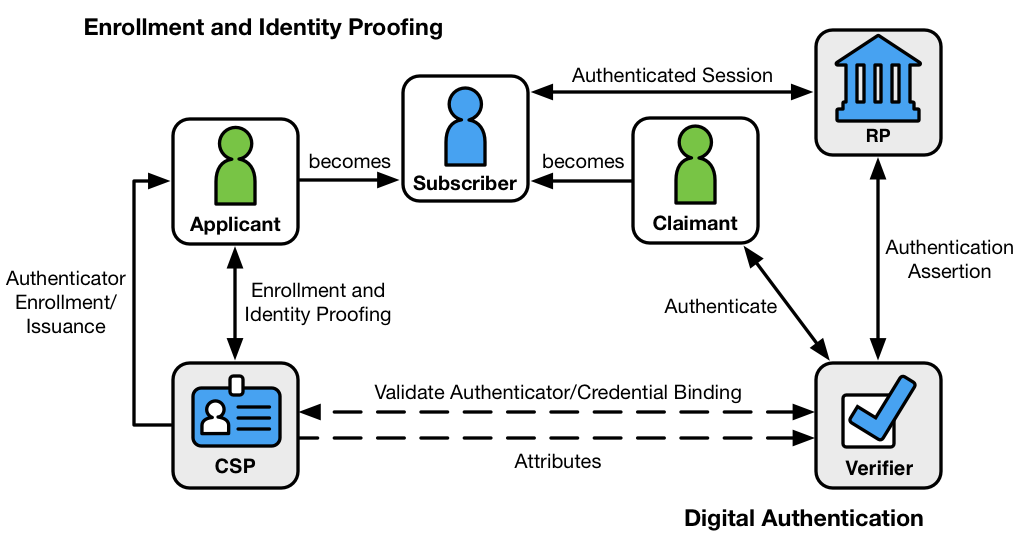
\includegraphics[width=.95\textwidth]{nist-model}
    \caption{Digital Identity Model. Taken from.
    % %REFERENCE Digital identity guidelines: revision 3
    }
    \label{fig:nist-model}
\end{figure}

\paragraph{SP 800-63A}
This volume of the Digital Identity Guidelines defines three Identity Assurance Levels (IALs) and requirements on identity proofing for each level. The \acrshort{ial}1 requires no verification of assertions provided by the user. \acrshort{ial}2 requires either remote or physically-present verification of assertions made by the user, while \acrshort{ial}3 requires manual verification by a trained person, representing the \acrshort{csp}/

% REFERENCE Digital identity guidelines: enrollment and identity proofing

\paragraph{SP 800-63B}
The B volume of the Guidelines defines three Authenticator Assurance Levels (AALs).

To authenticate themselves in AAL1, the user needs to demonstrate control of one authenticator. This must be done through a secure authentication protocol.

In AAL2, the user must demonstrate control of two distinct authenticators. This can be in a form of a multi-factor authenticator, or single-factor possession-based authenticator together with a memorised password. Cryptographic techniques defined in
% REFERENCE SECURITY REQUIREMENTS FOR CRYPTOGRAPHIC MODULES
must be used.

In AAL3, a hardware-based authenticator must be used in addition to requirements of AAL2. Furthermore, one of the authenticators used must be resistant to attacks attempting to impersonate the user.

\paragraph{SP 800-63C}

% TODO WRITE HERE

\paragraph{Authenticator types}
